\documentclass[dvipsnames]{../../../../AritzhClass}

\usepackage{array}

\izenburua{Nonograma}
\azpiizenburua{Proiektuaren Txostena}
\smalltitle{Nonograma: Txostena}
\ikasgaia{Ingeniaritza Informatikoa: KE}
\author{Aritz Lopez, Iñigo Arnedo eta Elena Hernández}
\data{\today}

\begin{document}

\izenburuorrialdea

\tableofcontents

\pagebreak

\section{Proiektuaren enuntziatua}

Nintendo DS-rako \textit{100 doors} jokuaren motako ate bat diseinatu eta programatu, DS-aren pantaila, teklatua eta denboragailua erabiliz.

\section{Proiektuaren definizioa: Nonograma}

Nonograma adimen joko japoniar bat da, Sudoku baten antzekoa, baina kasu honetan laukiak zenbakiekin bete beharrean, zenbaki konbinazio zehatz bat lortzeko, laukitxoak bete egin behar dira irudi zehatz bat lortzeko. Irudi zehatz hori lortu ahal izateko laukitxoak bete egin behar dira, eta laukitxo egokiak aukeratu ahal izateko goikaldean eta ezker aldean zenbaki batzuk aurkituko ditugu, horiek jarraian bete beharreko laukitxoen kopurua adierazten dute. Irudia aldez aurretik aukeratua da eta jokoa irabaztea ezinezkoa da beste irudiren bat lortu ezkero. 

\textit{100 doors} jokorako ate bat diseinatu behar genuenez, nonograma honetarako irudia giltza bat izatea adostu genuen, honen bitartez irekitzen baitira ateak. 

Jokoaren deskribapena:
Laguntza bezala, kontagailu bat agertzen da pantailan, honek adierazten digu zenbat laukitxo aldatu behar ditugun irudia zuzena izan dadin. Kontagailu hau inkrementatu egiten da zuzena den laukitxo bat ezabatu, edo okerra den bat bete ondoren, horrela ziurtatuta gelditzen da kontagailua ez dela 0-ra iritsiko irudi zuzena ez bada lortzen. 

Jokoa amaitzeko modu bakarra kontagailua 0-ra iristea da, hau da, irudi zuzena lortzea, eta horren ondoren irudiaren gainean sakatzea atea ireki ahal izateko. Behin irudia lortuta 10 segundu pasa eta gero irudiaren gainean ez bada sakatzen, jokoa berrabiarazi egingo da.

Jokoa hasi orduko, pantailako lauki guztiak txuriz agertuko dira. Lauki txuri baten gainean behin sakatuz gero, beltz bihurtuko da, eta alderantziz ere, hau da, lauki beltz baten gainean sakatuz gero, txuri bilakatuko da. 

Adibideak:

\begin{taula}{}{argazkiTaula}{cc}
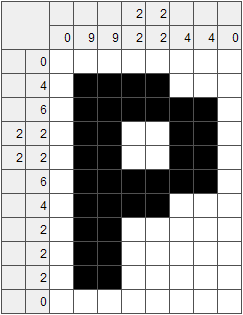
\includegraphics[scale=0.75]{nonograma1} & 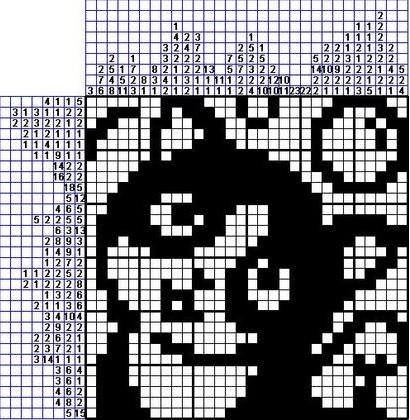
\includegraphics[scale=0.75]{nonograma2} \\
Adibide sinplea & Profesionalentzako bakarrik...
\end{taula}

\section{Kontzeptu-mapa}

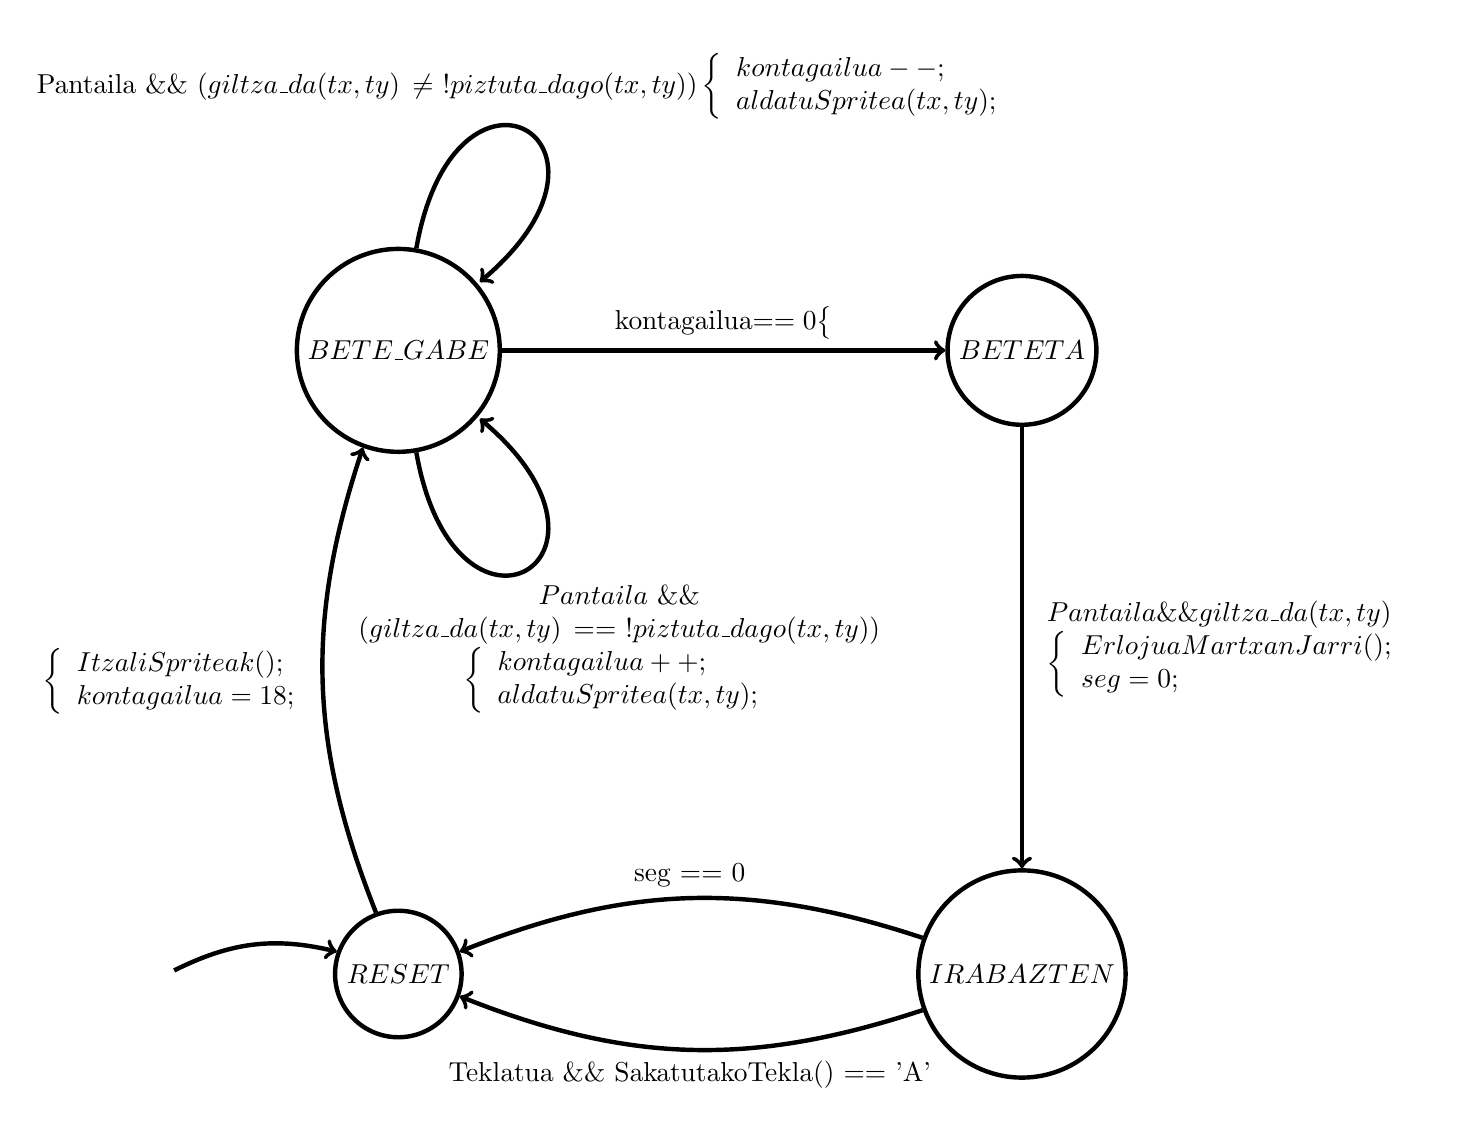
\begin{tikzpicture}[y=-1cm, scale=0.99, every node/.style={scale=0.99}]
\node(start) at (-3,8){};
\node(0) at (0,0)	[shape=circle,draw, ultra thick]	{$BETE\_GABE$};
\node(1) at (8,0)	[shape=circle,draw, ultra thick]	{$BETETA$};
\node(2) at (8,8)	[shape=circle,draw, ultra thick]	{$IRABAZTEN$};
\node(3) at (0,8)	[shape=circle,draw, ultra thick]	{$RESET$};
\path [ultra thick, ->]
  (start) edge [bend left=20] node [above] {} (3)
  (0) edge [in=40,out=80,loop] node [above] {Pantaila $\&\& \,\left(\text{giltza\_da}(tx, ty)\, \neq \,\, !\text{piztuta\_dago}(tx, ty)\right)\left\{\begin{array}{l}\text{kontagailua}--;\\ \text{aldatuSpritea(tx, ty);}\end{array}\right.$}
  (0) edge [in=320,out=280,loop] node [below right, xshift=-70] {$\begin{array}{c}\text{Pantaila} \,\, \&\& \\ \left(\text{giltza\_da}(tx, ty)\, == \,\, !\text{piztuta\_dago}(tx, ty)\right) \\ \left\{\begin{array}{l}\text{kontagailua}++;\\ \text{aldatuSpritea(tx, ty);}\end{array}\right.\end{array}$}
  (0) edge node [above] {kontagailua$==0 \big\{$} (1)
  (1) edge [below] node [right] {$\begin{array}{l}\text{Pantaila \&\& giltza\_da(tx, ty)} \\ \left\{\begin{array}{l}\text{ErlojuaMartxanJarri();}\\ \text{seg=0;}\end{array}\right.\end{array}$} (2)
  (2) edge [bend right=20] node [above] {seg == 0} (3)
  (2) edge [bend left=20] node [below] {Teklatua \&\& SakatutakoTekla() == 'A'} (3)
  (3) edge [bend left=20] node [left] {$\left\{\begin{array}{l}ItzaliSpriteak(); \\ kontagailua=18; \\ \end{array}\right.$} (0)
  ;
\end{tikzpicture}

\end{document}
